\chapter{Industrialisation du produit}
\label{Industrialisation du produit}
\thispagestyle{fancy}
Une fois le processus fonctionnel de notre système défini, on l'industrialise. Cela signifie que l'on crée un ensemble d'outils permettant de l'utiliser de la manière la plus simple possible et en répondant au mieux à la problématique initiale. \\
On soumet deux types d'outils: l'API, qui permet d'utiliser le système d'automatisation de l'investigation, et les outils graphiques, qui accompagnent l'usage de l'API et permettent à l'utilisateur d'interagir avec le programme.  

\section{API}
\label{Industrialisation du produit: API}
L'API que l'on propose est composée de 3 modules principaux:
\begin{description}
	\item [data base] Permet de gérer le stockage et la lecture des données nécessaires à l'exécution des algorithmes d'apprentissage. Deux types de fichiers sont sauvegardés dans la base de donnée: les fichiers logs, qui fournissent l'ensemble des exemples permettant d'entraîner l'algorithme et les fichiers générés par l'algorithme lors de son apprentissage.
	\item [data set] Gère le pré-traitement et le traitement des exemples afin de les structurer pour réaliser l'apprentissage par la suite.
	\item [machine learning] Permet de créer un algorithme d'apprentissage, de l'entraîner et de l'utiliser pour investiguer sur la root cause pour laquelle il a été créé.
\end{description}

La librairie utilise le langage de programmation Python \cite{Python}. \\

\subsection{Pré-traitement et traitement des données}
\label{Industrialisation du produit: API: Pré-traitement et traitement des données}
Le module "Data set" contenu dans l'API permet de pré-traiter les exemples et de les structurer afin de pouvoir réaliser l'apprentissage. 
Le pré-traitement est composé de 5 étapes.
\begin{description}
	\item [Lecture] La première étape du pré-traitement consiste à lire les données contenues dans le fichier log. 
	\item [Échantillonnage] Les fichiers logs générés par MEIGUI lors du déroulement du Filtering Test n'ont pas forcement tous la même période d'échantillonnage. Cela signifie que les exemples que l'on souhaite utiliser pour l'entraînement ne font pas tous la même taille. Or, les spécificités des fonctions de la librairie Scikit-learn utilisées pour l'entraînement nécessite que celles-ci aient le même nombre d'échantillons. Pour cette raison, échantillonne les données extraites des fichiers logs avec le même nombre d'échantillons. Si le nombre d'échantillons contenu dans le fichier log est inférieur au nombre d'échantillons fixé pour l'échantillonnage, on effectue un sur-échantillonnage lorsque celui-ci n'altère les données. 
	\item [Selection des motifs] Au regard de l'architecture fonctionnelle que l'on a définie en partie \ref{Automatisation du processus d'investigation: Achitecture High Level du système proposé}, on doit extraire les motifs caractéristiques d'une root cause dans chaque exemple utilisé. Pour cela, une sélection manuelle du motif est réalisée en amont via une interface graphique (c.f. \ref{Industrialisation du produit: Présentation des outils: Outils graphiques}). A partir des informations retournées par l'IHM, on est en mesure de sélectionner les données correspondant aux motifs, dans chacun de nos exemples. On rappelle que l'on enregistre également des morceaux de la courbe ne correspondant pas au motif d'une root cause, afin d'avoir les deux types de label lors de l'entrainement de l'algorithme.
	\item [Déroulement des données] On déroule ensuite les données afin de pouvoir réaliser de la reconnaissance de motifs sur plusieurs features (c.f. partie ) \ref{Automatisation du processus d'investigation: Étendre le problème à plusieurs dimensions}), i.e. que l'on place chacune des colonnes de notre matrice d'exemples l'une en dessous de l'autre pour obtenir en sortie un vecteur. 
	\item [Tri des données] Enfin, afin de pouvoir mesurer les performances de notre algorithme (c.f. partie \ref{Automatisation du processus d'investigation: Performances de la solution}), on sépare notre base de données d'exemples en deux groupes: le training set et le test set. Le premier sera utilisé pour entraîner notre algorithme, le deuxième pour le tester. 
\end{description}

\subsection{Sélection des motifs lors du pré-traitement des données }
\label{Industrialisation du produit: API: Sélection des motifs pour entrainement}
Comme étudié en partie \ref{Automatisation du processus d'investigation: Reconnaissance de motifs}, la reconnaissance de motifs passe par la sélection des motifs caractéristiques de la root cause que l'on souhaite détecter pour chaque exemple de notre base de donnée. Elle s'accompagne également de  la sélection de sections de la courbe ne présentant pas ce motif afin de pouvoir réaliser l'apprentissage de l'algorithme correctement( c.f. partie \ref{Automatisation du processus d'investigation: Difficultés notoires rencontrées}). Chaque motif sélectionné doit avoir la même taille i.e. le même nombre d'échantillons pour pouvoir réaliser l'entrainement. Cette taille dépend de la largeur globale du motif caractéristique de la root cause étudiée et est déterminée lors de l'utilisation de l'interface graphique présentée partie ... .   

\subsection{Format des données en sortie du pré-traitement des données}
\label{Industrialisation du produit: API: Format des données en sortie du pré-traitement}
On présente dans le tableau \ref {tab: Structure de la base de données d'exemples après prétraitement} la structure des données en sortie du pré traitement des données. On a deux vecteur : un contenant les exemples de motifs et un deuxième contenant le label associé à chaque motif. Le label 1 signifie que le motif lié correspond à un motif caractéristique de la root cause que l'on cherche à détecter; 0 signifie que le motif lié ne correspond pas à un motif caractéristique de la root cause que l'on cherche à détecter. 
\begin{equation}
\begin{blockarray}{cc}
exemples & label \\
\begin{block}{[c][c]}
exemple_1 &  1 \\
exemple_2 & 0 \\
exemple_3 & 0 \\
exemple_4 & 1 \\
... & ... \\
exemple_m & 0 \\
\end{block}
\end{blockarray}
\label {tab: Structure de la base de données d'exemples après prétraitement}
\end{equation}
On retrouve cette structure pour chaque \emph{set} (i.e. \emph{training set} et \emph{test set})
Chaque exemple correspond à une liste qui contient l'ensemble des échantillons contenus dans un motif (c.f. partie \ref{Industrialisation du produit: API: Sélection des motifs pour entrainement}).

\subsection{Module Marchine Learning et librairie scikit-learn}
\label{Industrialisation du produit:  API: Le module Machine Learning}
Le module Machine Learning s'appuie sur l'utilisation de scikit-learn \cite{ScikitLearn}. Il s'agit d'une bibliothèque Open Source développée par l'INRIA (Institut National de Recherche en Informatique et en Automatique \cite{INRIA}). Elle propose de nombreux outils afin de réaliser de la classification (régression logistique, SVM), de la régression (SVR, régression linéaire) et du clustering (i.e. apprentissage non supervisé). Elle est principalement utilisée dans notre cas pour réaliser de classification (i.e. apprentissage supervisé) en utilisant l'algorithme d'apprentissage automatique SVM. Elle est également utilisée afin de construire le \emph{training set} et le \emph{test set}.




\section{Outils graphiques}
\label{Industrialisation du produit: Outils graphiques}
On présente ici les différents outils graphiques permettant de réaliser la construction d'une nouvelle couche root cause (i.e. l'entrainement d'un nouvel algorithme à détecter une root cause particulière), d'investiguer un error name et d'obtenir des informations quant aux performances de l'algorithme. 

\subsection{Pattern selector}
\label{Industrialisation du produit: Outils graphiques: Pattern selection}
Cet outil graphique permet de sélectionner les motifs contenus dans chaque exemple du \emph{training set} durant la phase de pré-traitement des données. \\
Il est formé de trois parties:
\begin{item}
	- La première partie (encadré vert de la figure \ref{fig:Interface graphique du pattern selector}) nous donne divers indications sur l'état actuel du pré-traitement des données : la taille du motif actuellement sélectionné, le nom de l'exemple étudié et le nombre d'exemples restant à traiter. 
	- La seconde partie (encadré rouge de la figure  \ref{fig:Interface graphique du pattern selector}) est la partie graphique de l'interface graphique. Elle affiche les features de l'exemple actuellement étudiée. Dans le cas de la figure  \ref{fig:Interface graphique du pattern selector}, réalise par exemple l'entraînement de l'algorithme pour  que celui-ci puisse reconnaître le motif caractéristique de la root cause "frottement des freins de la hanche". La région en rouge permet de sélectionner le motif qui nous intéresse.
	- La dernière partie (encadré bleu de la figure  \ref{fig:Interface graphique du pattern selector}) est une succession de boutons permettant d'interagir avec les différents exemples.  
\end{item} 

\begin{figure}[h]
	\centering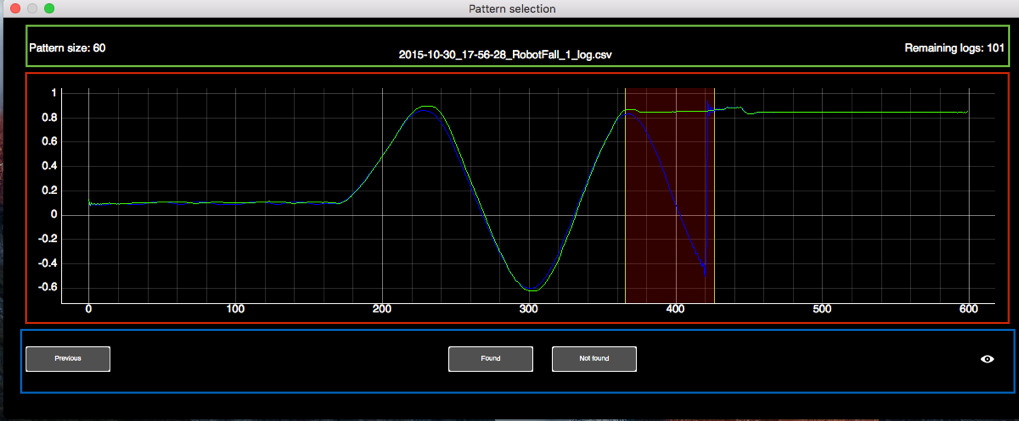
\includegraphics[height=6.4cm]{images/pattern_selector.png}
	\caption[Interface graphique du pattern selector]{Interface graphique du pattern selector.}
	\label{fig:Interface graphique du pattern selector}
\end{figure}

\begin{figure}[h]
	\centering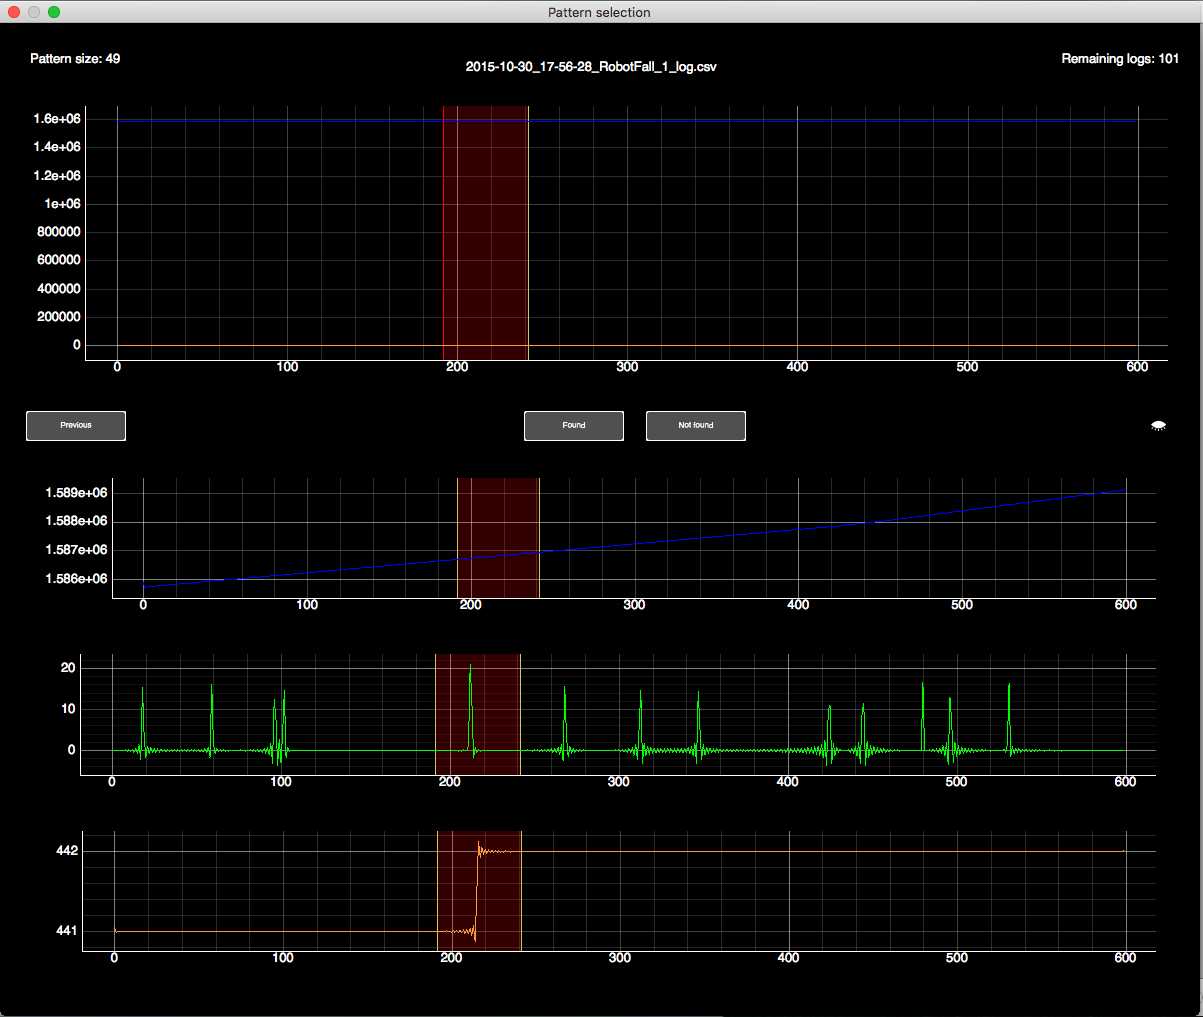
\includegraphics[height=7cm]{images/pattern_selector_ext.png}
	\caption[Interface graphique du pattern selector en mode étendu]{Interface graphique du pattern selector en mode étendue.}
	\label{fig:Interface graphique du pattern selector en mode étendu}
\end{figure}

\subsection{Probability visualization}
\label{Industrialisation du produit: Outils graphiques: Probability visualization}

\subsection{Control panel}
\label{Industrialisation du produit: Outils graphiques: Control panel}


\section{Utilisation suggérée des outils}
\label{Industrialisation du produit: Utilisation suggérée des outils}

\section{Dimensionnement de la solution}
\label{Industrialisation du produit: Dimensionnement de la solution}